\let\negmedspace\undefined
\let\negthickspace\undefined
\documentclass[journal,12pt,twocolumn]{IEEEtran}
\usepackage{float}
\usepackage{circuitikz}
\usepackage{cite}
\usepackage{amsmath,amssymb,amsfonts,amsthm}
\usepackage{algorithmic}
\usepackage{graphicx}
\usepackage{textcomp}
\usepackage{xcolor}
\usepackage{txfonts}
\usepackage{listings}
\usepackage{amsmath}
\usepackage{enumitem}
\usepackage{mathtools}
\usepackage{gensymb}
\usepackage{comment}
\usepackage[breaklinks=true]{hyperref}
\usepackage{tkz-euclide} 
\usepackage{listings}
\usepackage{gvv}                                        
\def\inputGnumericTable{}                                 
\usepackage[latin1]{inputenc}                                
\usepackage{color}                                            
\usepackage{array}                                            
\usepackage{longtable}                                       
\usepackage{calc}                                             
\usepackage{multirow}                                         
\usepackage{hhline}                                           
\usepackage{ifthen}                                           
\usepackage{lscape}
\newtheorem{theorem}{Theorem}[section]
\newtheorem{problem}{Problem}
\newtheorem{proposition}{Proposition}[section]
\newtheorem{lemma}{Lemma}[section]
\newtheorem{corollary}[theorem]{Corollary}
\newtheorem{example}{Example}[section]
\newtheorem{definition}[problem]{Definition}
\newcommand{\BEQA}{\begin{eqnarray}}
\newcommand{\EEQA}{\end{eqnarray}}
\newcommand{\define}{\stackrel{\triangle}{=}}
\theoremstyle{remark}
\newtheorem{rem}{Remark}

\renewcommand\thesection{\arabic{section}}
\renewcommand\thesubsection{\thesection.\arabic{subsection}}
\renewcommand\thesubsubsection{\thesubsection.\arabic{subsubsection}}

\renewcommand\thesectiondis{\arabic{section}}
\renewcommand\thesubsectiondis{\thesectiondis.\arabic{subsection}}
\renewcommand\thesubsubsectiondis{\thesubsectiondis.\arabic{subsubsection}}


\lstset{
language=Python,
frame=single, 
breaklines=true,
columns=fullflexible
}

\begin{document}
\bibliographystyle{IEEEtran}

\vspace{3cm}

\title{}
\author{EE23BTECH11020 -  Raghava Ganji \par Audio Filtering
}
\maketitle

\tableofcontents

\bigskip

\begin{abstract}
This manual provides a simple introduction to digital signal processing.
\end{abstract}

% \renewcommand{\thefigure}{\theenumi}
% \renewcommand{\thetable}{\theenumi}

\section{SOFTWARE INSTALLATION}
\bigskip

Run the following commands
\begin{lstlisting}
sudo apt-get update
sudo apt-get install libffi-dev libsndfile1 python3-scipy  python3-numpy python3-matplotlib 
sudo pip install cffi pysoundfile 
\end{lstlisting}

\section{Digital Filter}
\begin{enumerate}[label=\thesection.\arabic*
,ref=\thesection.\theenumi]
\item
\label{prob:input}
Download the sound file from 
\begin{lstlisting}
https://github.com/Raghava11020/Signals-and-Systems/blob/main/4/codes/RAF.wav
\end{lstlisting} 
\item
\label{prob:spectrogram}
You will find a Spectrogram at \href{https://academo.org/demos/spectrum-analyzer}{\url{https://academo.org/demos/spectrum-analyzer}}. 

Upload the sound file that you downloaded in Problem \ref{prob:input} in the spectrogram  and play.  Observe the Spectrogram. What do you find?\bigskip
\\
\solution There are a lot of yellow lines less than 440 .  These represent the synthesizer key tones. Also, the key strokes are audible along with background noise. It clearly shows that tonal frequency is under 500Hz. And above 500Hz only noise is present.\\
\newpage
\begin{figure}
    \centering
    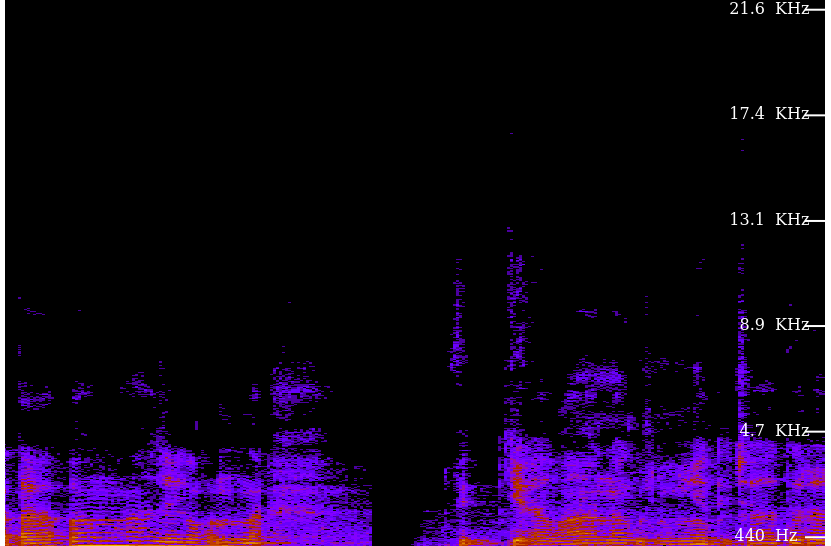
\includegraphics[width=0.85\linewidth]{figs/spectrogam_with_noise.png}
    \caption{spectrogram of original sound}
    \label{fig:spectrogram_with_noise}
\end{figure}
\item
\label{prob:output}

Write the python code for removal of out of band noise and execute the code.
\\
\solution
\begin{lstlisting}
import soundfile as sf
from scipy import signal
 
input_signal,fs = sf.read('keyboard.wav') 

sampl_freq=fs

order=4   

cutoff_freq=500.0  

Wn=2*cutoff_freq/sampl_freq  

b, a = signal.butter(order,Wn, 'low') 

output_signal = signal.lfilter(b, a, input_signal)

sf.write('Sound_With_ReducedNoise.wav', output_signal, fs) 
\end{lstlisting}

\item
The output of the python script in Problem \ref{prob:output} is the audio file Sound\_With\_ReducedNoise.wav. Play the file in the spectrogram in Problem \ref{prob:spectrogram}. What do you observe?\bigskip
\\
\solution The key strokes as well as background noise is subdued in the audio.  Also,  the signal is blank for frequencies above 500Hz.
\end{enumerate}
\section{DIFFERENCE EQUATION}
\begin{enumerate}[label=\thesection.\arabic*,ref=\thesection.\theenumi]
\item Let
\begin{equation}
x(n) = \cbrak{\underset{\uparrow}{1},2,3,4,2,1} \label{prob:2.1}
\end{equation}
Sketch $x(n)$. 
\item Let
\begin{multline}
y(n) + \frac{1}{2}y(n-1) = x(n) + x(n-2), 
\\
y(n) = 0, n < 0 \label{prob:2.2}
\end{multline}
Sketch $y(n)$.\\
Solve\\
\end{enumerate}
\end{document}

